\documentclass[10pt]{article}
\usepackage[utf8]{inputenc}

\usepackage{latexsym}
\usepackage{amssymb,amsmath,amsthm}
\usepackage{graphicx}
\usepackage{sgame}
\usepackage{color}
\usepackage{authblk}

\theoremstyle{remark}
\newtheorem*{remark}{Remark}

\usepackage[hidelinks]{hyperref}
\usepackage{empheq}
\usepackage{blkarray}
\usepackage{cancel}
\usepackage{enumerate}
\usepackage{times}
\usepackage{array}
\usepackage{lscape}
\usepackage{xcolor}

\usepackage[margin=1in]{geometry}
\newcommand{\newword}[1]{\textbf{\emph{#1}}}

%Arrows
\newcommand{\into}{\hookrightarrow}
\newcommand{\onto}{\twoheadrightarrow}

%Things LaTeX names by appearance, rather than meaning
\newcommand{\isom}{\cong} %The isomorphism symbol
\newcommand{\union}{\cup}
\newcommand{\intersection}{\cap}
\newcommand{\bigunion}{\bigcup}
\newcommand{\bigintersection}{\bigcap}
\newcommand{\disjointunion}{\sqcup}
\newcommand{\bigdisjointunion}{\bigsqcup}

\newcommand\numberthis{\addtocounter{equation}{1}\tag{\theequation}}

%Some multiletter functions
\DeclareMathOperator{\Hom}{Hom}
\DeclareMathOperator{\Ext}{Ext}
\DeclareMathOperator{\End}{End}
\DeclareMathOperator{\Tor}{Tor}
\DeclareMathOperator{\Ker}{Ker}
\DeclareMathOperator{\CoKer}{CoKer}
\DeclareMathOperator{\Spec}{Spec}
\DeclareMathOperator{\Proj}{Proj}
\renewcommand{\Im}{\mathop{\mathrm{Im}}}
%Their calligraphic versions; use these for the sheaf constructions
\DeclareMathOperator{\HHom}{\mathcal{H} \textbf{om}}
\DeclareMathOperator{\EExt}{\mathcal{E} \textbf{xt}}
\DeclareMathOperator{\EEnd}{\mathcal{E} \textbf{nd}}
\DeclareMathOperator{\TTor}{\mathcal{T} \textbf{or}}
\DeclareMathOperator{\KKer}{\mathcal{K}\textbf{er}}
\DeclareMathOperator{\CCoKer}{\mathcal{C} \textbf{o}\mathcal{K} \textbf{er}}
\newcommand{\IIm}{\mathop{\mathcal{I} \textbf{m}}}
\newcommand{\ccH}{\mathscr{H}} %The very curly H

\DeclareMathOperator{\sss}{\mathrm{sunny}}
\DeclareMathOperator{\rrr}{\mathrm{rainy}}
\DeclareMathOperator{\hhh}{\mathrm{hot}}
\DeclareMathOperator{\ccc}{\mathrm{cold}}

%This makes alternating tensors look right in displayed equations
\newcommand{\Alt}{\bigwedge\nolimits}

%Blackboard bold letters
\renewcommand{\AA}{\mathbb{A}}
\newcommand{\BB}{\mathbb{B}}
\newcommand{\CC}{\mathbb{C}}
\newcommand{\DD}{\mathbb{D}}
\newcommand{\EE}{\mathbb{E}}
\newcommand{\FF}{\mathbb{F}}
\newcommand{\GG}{\mathbb{G}}
\newcommand{\HH}{\mathbb{H}}
\newcommand{\II}{\mathbb{I}}
\newcommand{\JJ}{\mathbb{J}}
\newcommand{\KK}{\mathbb{K}}
\newcommand{\LL}{\mathbb{L}}
\newcommand{\MM}{\mathbb{M}}
\newcommand{\NN}{\mathbb{N}}
\newcommand{\OO}{\mathbb{O}}
\newcommand{\PP}{\mathbb{P}}
\newcommand{\QQ}{\mathbb{Q}}
\newcommand{\RR}{\mathbb{R}}
\renewcommand{\SS}{\mathbb{S}}
\newcommand{\TT}{\mathbb{T}}
\newcommand{\UU}{\mathbb{U}}
\newcommand{\VV}{\mathbb{V}}
\newcommand{\WW}{\mathbb{W}}
\newcommand{\XX}{\mathbb{X}}
\newcommand{\YY}{\mathbb{Y}}
\newcommand{\ZZ}{\mathbb{Z}}

%Calligraphic letters

\newcommand{\cA}{\mathcal{A}}
\newcommand{\cB}{\mathcal{B}}
\newcommand{\cC}{\mathcal{C}}
\newcommand{\cD}{\mathcal{D}}
\newcommand{\cE}{\mathcal{E}}
\newcommand{\cF}{\mathcal{F}}
\newcommand{\cG}{\mathcal{G}}
\newcommand{\cH}{\mathcal{H}}
\newcommand{\cI}{\mathcal{I}}
\newcommand{\cJ}{\mathcal{J}}
\newcommand{\cK}{\mathcal{K}}
\newcommand{\cL}{\mathcal{L}}
\newcommand{\cM}{\mathcal{M}}
\newcommand{\cN}{\mathcal{N}}
\newcommand{\cO}{\mathcal{O}}
\newcommand{\cP}{\mathcal{P}}
\newcommand{\cQ}{\mathcal{Q}}
\newcommand{\cR}{\mathcal{R}}
\newcommand{\cS}{\mathcal{S}}
\newcommand{\cT}{\mathcal{T}}
\newcommand{\cU}{\mathcal{U}}
\newcommand{\cV}{\mathcal{V}}
\newcommand{\cW}{\mathcal{W}}
\newcommand{\cX}{\mathcal{X}}
\newcommand{\cY}{\mathcal{Y}}
\newcommand{\cZ}{\mathcal{Z}}


\DeclareMathOperator{\ord}{ord}
\DeclareMathOperator{\inte}{int}
\DeclareMathOperator{\nhd}{nhd}

\newcommand{\ds}{\displaystyle}
\newcommand{\mc}{\mathcal}
\newcommand{\ol}{\overline}
\newcommand{\modu}{\hspace{-2mm} \mod}

\DeclareMathOperator{\inn}{Inn}
\DeclareMathOperator{\aut}{Aut}
\DeclareMathOperator{\cen}{Center}
\DeclareMathOperator{\im}{Im}
\DeclareMathOperator{\re}{Re}
\DeclareMathOperator{\id}{id}
\DeclareMathOperator{\mor}{Mor}
\DeclareMathOperator{\irr}{Irr}
\DeclareMathOperator{\sgn}{sgn}

\DeclareMathOperator{\cov}{Cov}
\DeclareMathOperator{\var}{Var}

\DeclareMathOperator{\erf}{erf}
%\DeclareMathOperator{\sgn}{sgn}
\DeclareMathOperator{\argmin}{argmin}
\DeclareMathOperator{\argmax}{argmax}

\DeclareMathOperator{\lip}{Lip}

\newcommand{\bbm}{\begin{bmatrix}}
\newcommand{\bpm}{\begin{pmatrix}}
\newcommand{\ebm}{\end{bmatrix}}
\newcommand{\epm}{\end{pmatrix}}

\newcommand{\ddx}[2]{\frac{d #1}{d #2}}
\newcommand{\ddt}[1]{\frac{d #1}{dt}}

 \newcommand{\del}[2]{\frac{\partial #1}{\partial #2}}
 \newcommand{\dsdel}[2]{\displaystyle\frac{\partial #1}{\partial #2}}
 
 \newcommand{\doubledel}[3]{\displaystyle\frac{\partial^2 #1}{\partial #2 \partial #3}}
 \newcommand{\doubledelsame}[2]{\displaystyle\frac{\partial^2 #1}{\partial #2^2}}
  
%newcommand{\ddx}[2]{\frac{d #1}{d #2}}
%\newcommand{\ddt}[1]{\frac{d #1}{dt}}

\newcommand{\dsddx}[2]{\displaystyle\frac{d #1}{d #2}}
\newcommand{\dsddt}[1]{\displaystyle\frac{d #1}{dt}}

\newcommand{\pbderiv}{\ds\del{V}{n_1} \dsddt{n_1} + \ds\del{V}{n_2} \dsddt{n_2}}

\newcommand{\ito}{It\^o \hspace{0.05mm}}
\newcommand{\itos}{It\^os \hspace{0.05mm}}

\newcommand{\gronwall}{Gr\"onwall  \hspace{0.05mm}}
\newcommand{\gronwalls}{Gr\"onwall's  \hspace{0.05mm}}

\newcommand{\tw}{d\tilde{W}_t}
\newcommand{\tws}{d\tilde{W}_s}

\newcommand{\A}{{\color{red}A}}
\newcommand{\B}{{\color{blue}B}}

\bibliographystyle{plain}
\usepackage{float}


%%%%%%%%%%%%%%%%%%%%%%%%%%%
% Document-specific settings

\title{\LARGE Analytical Mixing Model, v2\vspace{-10pt}}
\author{Mari Kawakatsu\vspace{-15pt}}
\date{Last updated: \today\vspace{-15pt}}

\graphicspath{ {../output/Task_dist/} }
\usepackage[margin=.2in]{caption}

%%%%%%%%%%%%%%%%%%%%%%%%%%%
\begin{document}

\maketitle

\tableofcontents
% \vspace{30pt}
\section{Overview}
\begin{itemize}
    \item Following up on the last Skype with Yuko \& Daniel, I ran additional simulations in which I varied a combination of parameters, namely the task efficiencies $\alpha$ and the demand rates $\delta$ (results on slides).
    
    \item There seemed to be some strange behavior when at least one of the lines was inefficient. To understand what was happening, I decided to write down equations that approximate the computational model to gain insight into the (expected) steady-state behavior (see Sections~\ref{sec:model} and \ref{sec:ss}).
    
    \item A preliminary analysis of the model seems to suggest that, assuming that the system reaches/has a steady state, varying only $\delta$ and $\alpha$ can result in a downward contagion but not an upward contagion (see Section~\ref{sec:contagion}). If this is true, then in order for the FTM to capture the experimental data, it must be the case that the two genetic lines differ in some trait other than their task efficiency.
    
    \item (Update 2/9) I extended the model to capture non-50-50 mixes.
    
\end{itemize}

\section{Model} \label{sec:model}

To consider the dynamics of division of labor in mixed colonies, we extend the fixed threshold model in \cite{ulrich18} to incorporate ants of two genetic lines, \A\ and \B. 

The model considers $n$ individuals and $m$ tasks. 
{\color{orange}Let $f$ and $1-f$ be the fractions of genetic line \A\ and \B\ individuals in the colony, respectively.}
% The $n$ individuals consist of equal numbers of genetic line \A\ and genetic line \B\ individuals.
We assume that each task $j$ has an associated stimulus, $s_{j,t}$, at every time $t$, indicating group-level demand for that task. We model the change in stimulus over discrete time as
\begin{equation}
    s_{j,t+1} - s_{j,t} = \delta_j - \frac{\alpha_j^{\A} n_{j,t}^{\A} + \alpha_j^{\B} n_{j,t}^{\B} }{n}, \label{eq:stim}
\end{equation}
where 
\begin{itemize}
    \item $\delta_j$ is the task-specific demand rate;
    \item $\alpha_j^{\A}$ and $\alpha_j^{\B}$ are the task-specific performance efficiencies of lines \A\ and \B, respectively; and
    \item $n_{j,t}^{\A}$ and $n_{j,t}^{\B}$ are the numbers of line \A\ and line \B\ individuals performing task $j$ and time $t$, respectively.
\end{itemize}

At each time step, inactive individuals are exposed to the task stimuli randomly until either they begin performing a task or they have encountered all stimuli without landing on a task. Similar to \cite{ulrich18}, our computational model draws individual $i$'s internal threshold for task $j$, $\theta_{ij}$, from a normal distribution with mean $\mu_j$ and normalized standard deviation $\sigma_j$ (each of these parameters can be line- and/or task-specific). \textit{To gain analytical insight into the model, we make the simplifying assumption that the line- and task-specific thresholds are given by the constant parameters, $\mu_j^{\A}$ and $\mu_j^{\B}$.}

With this assumption, the probabilities $P_{ij,t}^{\A}$ and $P_{ij,t}^{\B}$ that individuals $i$ of lines \A\ and \B, respectively, perform task $j$ at time $t$ can be written as
\begin{equation}
    P_{j,t}^{\A} (s_{j,t}) = \frac{s_{j,t}^\eta}{s_{j,t}^\eta + {(\mu_j^{\A})}^\eta}, \quad P_{j,t}^{\B} (s_{j,t}) = \frac{s_{j,t}^\eta}{s_{j,t}^\eta +{(\mu_j^{\B})}^\eta},
\end{equation}
where $\eta$ is the threshold response parameter as in the original model. Finally, at a given time $t$, active individuals quit their tasks with a constant quit probability $\tau$. In the case of two tasks ($m = 2$), the change in the number of line \A\ and line \B\ individuals working on task $j$ is given by\footnote{explain this more in English}
\begin{align}
    n_{j,t+1}^{\A} - n_{j,t}^{\A} & = \frac{1}{2} \bigg[ P_{j,t}^{\A}(s_{j,t}) + (1 - P_{j',t}^{\A}(s_{j',t}))P_{j,t}^{\A}(s_{j,t})\bigg] \bigg( {\color{orange}fn}
 - (n_{j,t}^{\A} + n_{j',t}^{\A}) \bigg) - \tau n_{j,t}^{\A} \nonumber\\
    n_{j,t+1}^{\B} - n_{j,t}^{\B} & = \frac{1}{2} \bigg[ P_{j,t}^{\B}(s_{j,t}) + (1 - P_{j',t}^{\B}(s_{j',t}))P_{j,t}^{\B}(s_{j,t})\bigg] \bigg( {\color{orange}(1-f)n} - (n_{j,t}^{\B} + n_{j',t}^{\B}) \bigg) - \tau n_{j,t}^{\B} \label{eq:active}
\end{align}
for $(j,j')=(1,2), (2,1)$. {\color{black}The sums in square brackets capture the possible ways in which individuals can initiate task $j$: they can either encounter the stimulus for task $j$ immediately and begin performing that task, or they can first encounter the stimulus for the other task $j'$, decide not to perform that task, subsequently encounter the stimulus for task $j$, and begin performing task $j$.}

The full model for $m=2$ consists of the six equations describing changes in $s_1, s_2$ \eqref{eq:stim} and $ n_1^{\A}, n_1^{\B}, n_2^{\A}, n_2^{\B}$ \eqref{eq:active}. Given initial conditions 
% $s_{1,0} \geq 0$, $s_{2,0} \geq 0$, 
$0\leq n_{1,0}^{\A}+n_{2,0}^{\A} \leq fn$ and $0\leq n_{1,0}^{\B}+ n_{2,0}^{\B} \leq (1-f)n$,
the dynamics will satisfy the constraints $0\leq n_{1,t}^{\A}+n_{2,t}^{\A} \leq fn$ and $0\leq n_{1,t}^{\B}+ n_{2,t}^{\B} \leq (1-f)n$ for all $t \geqq 0$.


\begin{proof}[Proof sketch]
Here we only consider the case for line \A, but the proof for line \B\ is analogous.

Consider the dynamics of $X_{t}^{\A} \equiv n_{1,t}^{\A}+n_{2,t}^{\A}$, given by
\begin{align*}
    X_{t+1}^{\A} & = n_{1,t+1}^{\A}+n_{2,t+1}^{\A} \\
    &= (1-\tau)(n_{1,t}^{\A}+n_{2,t}^{\A}) + \frac{1}{2}
    \bigg[ 2P_{1,t}^{\A}(s_{1,t}) + 2P_{2,t}^{\A}(s_{2,t}) - 2 P_{1,t}^{\A}(s_{1,t}) P_{2,t}^{\A}(s_{2,t})\bigg] \\
    &= (1-\tau)(X_{t}^{\A}) + 
    \bigg[ P_{1,t}^{\A}(s_{1,t}) + P_{2,t}^{\A}(s_{2,t}) -  P_{1,t}^{\A}(s_{1,t}) P_{2,t}^{\A}(s_{2,t})\bigg]
    \big( fn - X_{t}^{\A} \big)
\end{align*}
Now, let
\begin{align*}
    K_{t} \equiv P_{1,t}^{\A}(s_{1,t}) + P_{2,t}^{\A}(s_{2,t}) -  P_{1,t}^{\A}(s_{1,t}) P_{2,t}^{\A}(s_{2,t}).
\end{align*}
Since $0 \leq P_{1,t}^{\A}(s_{1,t}), P_{2,t}^{\A}(s_{2,t}) \leq 1$ for all\footnote{What guarantees this condition? Can it be violated?} $ s_{1,t}, s_{2,t} \geq 0$, we have that $0\leq K_t \leq 1$ for all $t\geq 0$. Then,
\begin{align}
    0\leq X_{t}^{\A} \leq fn \quad\Longrightarrow\quad X_{t+1}^{\A} = (1-\tau)(X_{t}^{\A}) + 
    K_{t}\cdot\big( fn - X_{t}^{\A} \big) \leq -\tau X_{t}^{\A} + fn \leq fn. \label{eq:induction}
\end{align}
In other words, at time $t+1$, $0\leq n_{1,t+1}^{\A}+n_{2,t+1}^{\A} = X_{t+1}^{\A} \leq fn$ always holds provided that the same condition is satisfied at time $t$.
A formal proof of the statement(s) require an induction on $t$ using the inequality \eqref{eq:induction}.
\end{proof}

\section{Steady-state predictions} \label{sec:ss}
One way to understand what is happening in the simulations is to consider the equilbria of the above model. My intent here is not (yet) to prove the stability etc. rigorously but to get a sense for what we should expect to see in the simulations.

\subsection{Pure colonies: 2 tasks, 1 line}
For pure (\A-only) colonies, we set $f = 1$ and $n_{j,t}^{\B} = 0$ for all time $t$. Setting Eq.~\eqref{eq:stim} to zero, we obtain
\begin{equation}
    \frac{n_j^{\A}}{n} = \frac{\delta_j}{\alpha_j^{\A}}
    \label{eq:ss1}
\end{equation}
as the fraction of (\A) ants that are performing task $j$ ($j = 1,2$) at steady state. We can us this to compute the steady-state levels of stimuli if needed.

\textbf{Notably, the steady-state values of $n_j^{\A}$ are \textbf{independent} of the mean threshold ($\mu_j^{\A}$) or the quit probability ($\tau^{\A}$)}. This agrees with the results of our simulations, where varying $\mu$ and $\tau$ by line did not lead to differing mean task performance levels in the pure colonies.

Note that the sum of the fractions \eqref{eq:ss1} across tasks should not exceed one. So a necessary condition for the steady-state to be biologically realizable is 
\begin{equation}
    \frac{n_1^{\A}}{n} + \frac{n_2^{\A}}{n} = \frac{\delta_1}{\alpha_1^{\A}} + \frac{\delta_2}{\alpha_2^{\A} }\leq 1 \label{eq:cond1}.
\end{equation}
If this condition is not met, then we would expect the stimuli to continue growing (i.e., the system will not reach a steady state). \textbf{A ``symptom'' of this phenomenon, I think, is that the ants become ``maxed out'' (I can explain this more when we Skype)}.

\subsection{Mixed colonies: 2 tasks, 2 lines, 50-50 mixes} \label{sec:5050}

{\color{black}We first consider the 50-50 mixes ($f=0.5$), i.e., mixed colonies consisting of an equal number of \A\ and \B\ ants.}
Moreover, we assume that the mean thresholds and the quit probabilities are identical for both tasks and lines ($\mu_1^{\A} = \mu_2^{\A} = \mu_1^{\B} = \mu_2^{\B}$ and $\tau^{\A} = \tau^{\B}$), as we have done in the simulations with varied $\delta$ and $\alpha$ values. Setting Eq.~\eqref{eq:stim} and Eq.~\eqref{eq:active} equal to zero, we find\footnote{This is the expression I get when I set $1\leq \eta \leq 20, \eta \in \ZZ$. There seems to be something numerically tricky when $\eta$ takes non-integer values.} the expression for the steady-state numbers of individuals performing task $j$:%\footnote{}
\begin{equation}
     n_j^{\A} =  n_j^{\B} = n\bigg(\frac{\delta_j}{\alpha_j^{\A} + \alpha_j^{\B}}\bigg) \label{eq:ss2a}
\end{equation}
for $j = 1, 2$.
Alternatively, as fractions of each genetic type of individuals,
\begin{equation}
     \frac{n_j^{\A}}{(n/2)} =  \frac{n_j^{\B}}{(n/2)} = \frac{2\delta_j}{\alpha_j^{\A} + \alpha_j^{\B}}. \label{eq:ss2}
\end{equation}
The necessary condition for this steady state to exist is
\begin{equation}
     \sum_{j=1}^2 \frac{n_j^{\A}}{n} + \frac{n_j^{\B}}{n} 
     = \sum_{j=1}^2 \frac{2\delta_j}{\alpha_j^{\A} + \alpha_j^{\B}}
     \leq 1.
     \label{eq:cond2}
\end{equation}
Again, if this condition is not met, then we would expect the stimuli to continue growing over time and for the ants to be working at max capacity.

While $\mu$ doesn't explicitly appear in \eqref{eq:ss2} when we assume that the mean thresholds are identical for all individuals and both tasks, we expect\footnote{I haven't been able to get Mathematica to compute the expressions explicitly, but we can infer this from the form of the threshold functions.} the general form of steady state fractions of active individuals to be functions of $\mu_j^{\A}$ and $\mu_j^{\B}$ as well as $\tau^{\A}$ and $\tau^{\B}$. \textbf{So one question to investigate using simulations (numerical or computational) would be \textbf{how the mean thresholds ($\mu$) interact with either the demand rates ($\delta$) or the task efficiencies ($\alpha$)}.}

\subsubsection{Comparing with simulation results}

\begin{figure}[H]
    \centering
    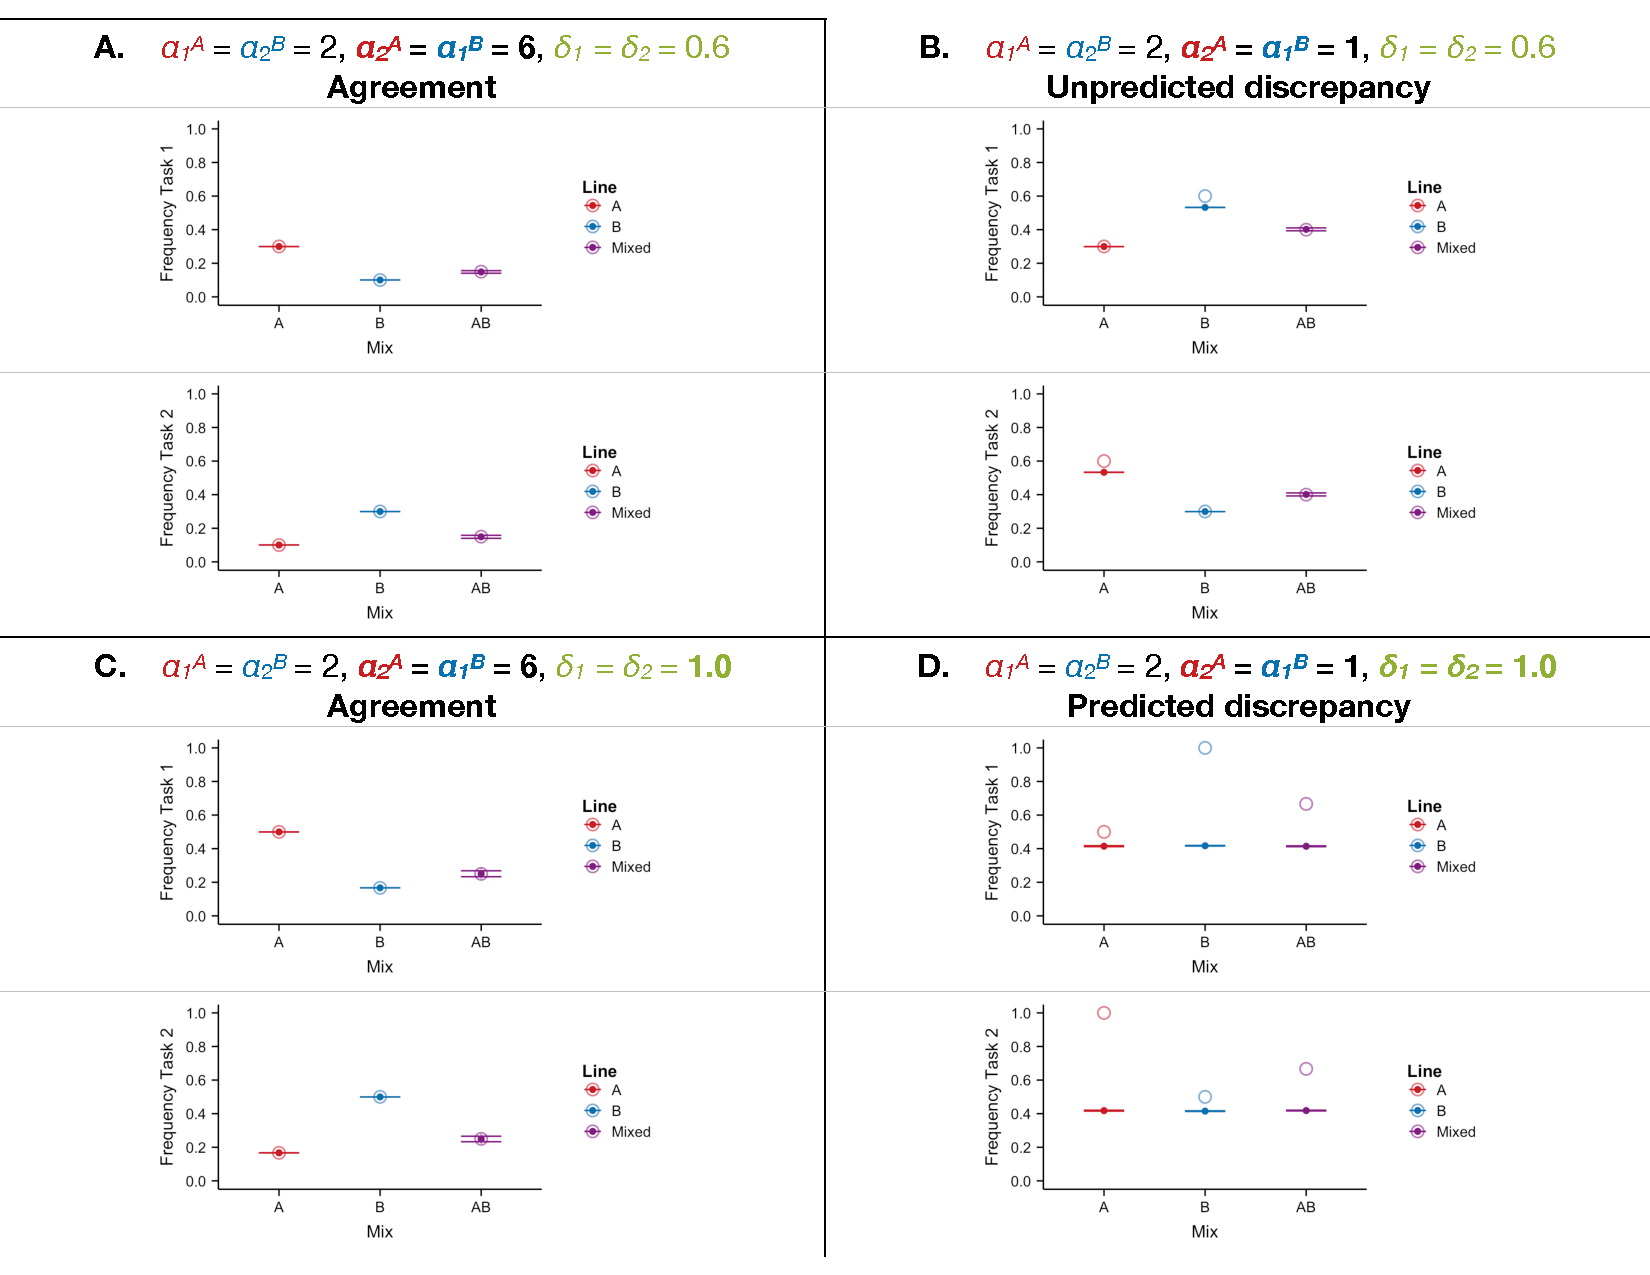
\includegraphics[trim={0 0.25in 0 0.2in}, clip, width=0.9\linewidth]{output/Task_dist/5050_comparison.pdf}
    \caption{Comparison of simulation results (solid dots with error bars) and analytical predictions of steady states (opaque rings). The following parameters are shared among the four cases (\textbf{A}-\textbf{D}): $\mu = 10, \sigma = 0.1, \eta = 7$. The other parameters are as indicated in the figure: the top row (\textbf{A} and \textbf{B}) has $\delta = 0.6$ while the bottom row (\textbf{C} and \textbf{D}) has $\delta = 1.0$; the left column (\textbf{A} and \textbf{C}) has super-efficient ants (with $\alpha = 6$) while the right column (\textbf{B} and \textbf{D}) has inefficient ants (with $\alpha = 1$). \textbf{Case A and C}: The model predictions of steady state task performance frequencies agree with simulation results. \textbf{Case D}: The model predictions and simulation results disagree in all cases, but the discrepancy was expected: since conditions \eqref{eq:cond1} (for pure colonies) and \eqref{eq:cond2} (for mixed colonies) are violated, we do not expect the system to be in equilibrium in the first place (in particular, the stimuli keep growing). \textbf{Case B}: The model overpredicts the steady-state task performance frequencies for the tasks at which the ants are less efficient (i.e., Task 2 for \A\ and Task 1 for \B), but in all other cases the model agrees with the simulation results.}
    \label{fig:5050_comp}
\end{figure}
\vspace{-5pt}
\textbf{Overall, the model performs well against the simulations when all the ants in the colony are sufficiently efficient (Fig.~\ref{fig:5050_comp}, left column). However, when some ants are inefficient (right column), the model overestimates the activity for the less efficient line, \textit{even when the system reaches a steady state} (\textbf{Case B} in Fig.~\ref{fig:5050_comp}).} Potential causes of this discrepancy might be:
\begin{itemize}
    \item We assumed that the threshold $\mu$ is constant for every genetic line and task, i.e., that there is no variation ($\sigma = 0$). {\color{orange}When I set $\sigma = 0$ in one set of simulations, however, the discrepancy did not go away. Plus we know from previous restuls that $\sigma$ only affects the variance in task performance, not the mean.}
    
    \item The analytical model does not explicitly take into account the fact that, in the simulations, an ant must be inactive for one time step before it can start a task. {\color{orange}This seems more likely, but I'm not yet sure how to incorporate this into the model.}
    
    \item {\color{orange}What else is missing??}
    
\end{itemize}

\subsection{Mixed colonies: 2 tasks, 2 lines, non-50-50 mixes (NEW)}

We now generalize to the case in which a fraction $f$ of individuals in a mixed colony are of genetic line \A. In the simplified case where $\mu_1^{\A} = \mu_2^{\A} = \mu_1^{\B} = \mu_2^{\B}$ and $\tau^{\A} = \tau^{\B}$, the steady-state fractions of individuals performing task $j$ are
\begin{equation}
     n_j^{\A} =  \frac{fn\delta_j}{f\alpha_j^{\A} + (1-f)\alpha_j^{\B}}, 
     \quad
     n_j^{\B} =  \frac{(1-f)n\delta_j}{f\alpha_j^{\A} + (1-f)\alpha_j^{\B}}, 
     \label{eq:ss3a}
\end{equation}
or, as fractions of the individuals of each genetic type (recall that there are $fn$ individuals of type \A\ and $(1-f)n$ individuals of type \B),
\begin{equation}
     \frac{n_j^{\A}}{fn} =  \frac{n_j^{\B}}{(1-f)n} = \frac{\delta_j}{f\alpha_j^{\A} + (1-f)\alpha_j^{\B}} \ \bigg(= \frac{n_j^{\A} + n_j^{\B}}{n}\bigg). \label{eq:ss3}
\end{equation}
The last equality highlights the fact that the fraction of individuals \textit{of each type} performing task $j$ is identical to the fraction \textit{of the whole colony} performing that task. As expected, the expressions \eqref{eq:ss3} reduce to \eqref{eq:ss2} when $f=0.5$ (50-50 mixes) and to \eqref{eq:ss1} when $f=1$ (pure \A\ colonies).

Again, we would expect to see this equilibria only when $n_1^{\A} + n_1^{\B} + n_2^{\A}+ n_2^{\B} \leq n$ is satisfied.

From these results, we would expect the steady-state fraction of task $j$ performance frequency (which corresponds to \eqref{eq:ss3}) to depend \textbf{nonlinearly} on the fraction of \A\ individuals ($f$). \\

\subsubsection{Comparing with simulation results}
\begin{figure}[H]
    \centering
    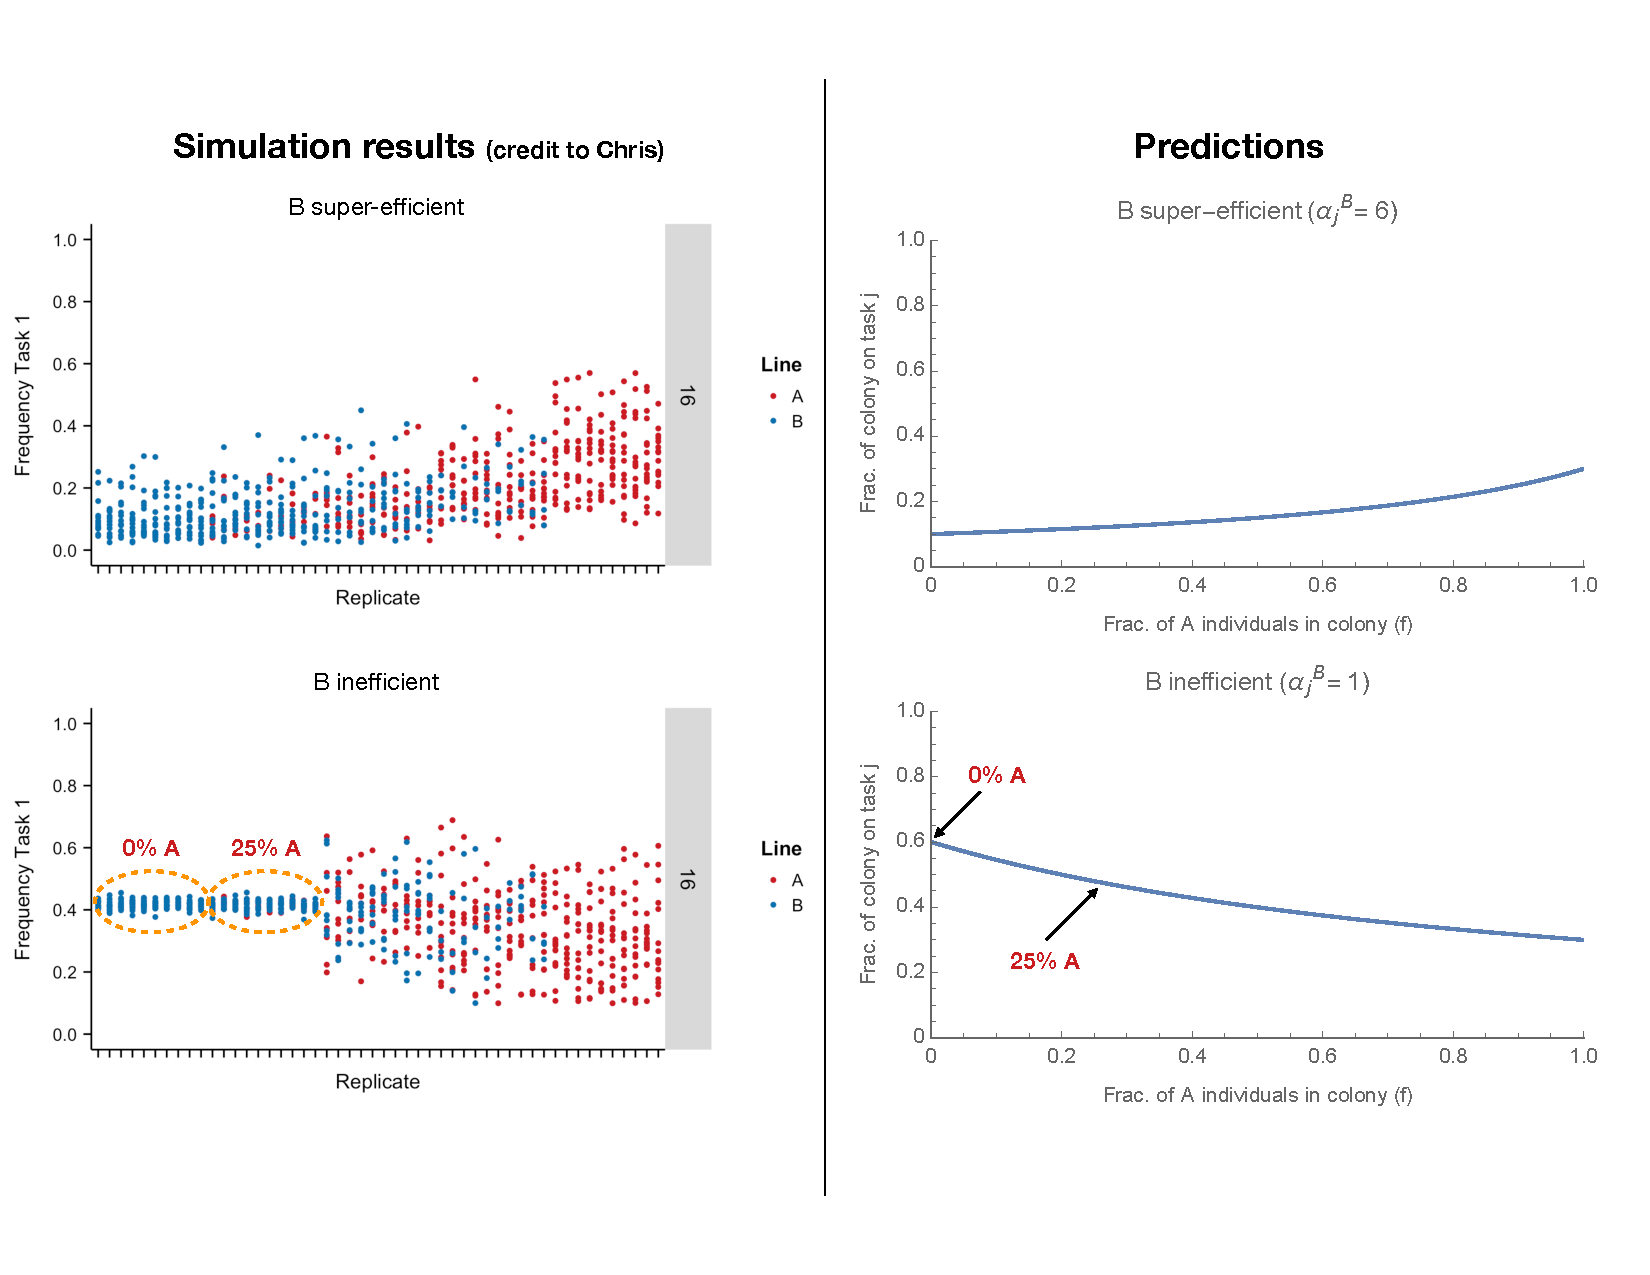
\includegraphics[trim={0 1in 0 0.75in}, clip, width=0.9\linewidth]{output/Task_dist/mixes_comparison.pdf}
    \caption{Comparison of simulation results (left) and analytical predictions of steady states (right) according to the model above. The parameters used in both columns are as follows: $\alpha_1^{\A} = \alpha_2^{\A} = 2, \delta= 0.6, \mu=10, \sigma = 0.1, \eta = 7$. 
    \textbf{Top row}: The \B\ ants are ``super-efficient'' at both tasks ($\alpha_1^{\B} = \alpha_2^{\B} = 2$, top row). In the simulations, task performance \textit{increases nonlinearly} as the fraction of \A\ ants in the colony increases (left), as predicted qualitatively by the model (right).
    \textbf{Bottom row}: The \B\ ants are ``inefficient'' at both tasks ($\alpha_1^{\B} = \alpha_2^{\B} = 1$). 
    Similar to the 50-50 cases, when the colony primarily consists of the inefficient \B\ ants ($f = 0, 0.25$ in the simulations), the model \textit{overpredicts} the colony activity.
    Where there are sufficiently many \A\ ants in the colony ($f = 0.5, 0.75, 1$ in the simulations), however, both the simulations and model predictions show a \textit{nonlinear negative} relationship in task performance.}
    \label{fig:mixes_comp}
\end{figure}

\subsection{Mixed colonies: 2 tasks, 2 lines, 50-50 mixes, symmetric task thresholds (NEW 2/15)}

In Section~\ref{sec:5050}, we assumed that the mean thresholds $\mu_{j}^{\A}$ and $\mu_{j}^{\B}$ were identically for both lines and tasks ($\mu_{1}^{\A} = \mu_{2}^{\A} = \mu_{1}^{\B} = \mu_{2}^{\B}$)
and derived steady-state fractions of individuals performing the two tasks. Notably, such fractions were independent of $\mu_{j}$ and dependent only on $\delta_j$ and $\alpha_{j}$.  To understand the full dynamics of the model, however, we also need to study \textbf{how the mean thresholds $\mu_{j}^{\A}$ and $\mu_{j}^{\B}$ affect the steady states}.

Below are the set of 6 equations describing the dynamics, assuming 50-50 mixes ($f=0.5$).
\begin{align}
    s_{1,t+1} - s_{1,t} & = \delta_1 - \frac{\alpha_1^{\A} n_{1,t}^{\A} + \alpha_1^{\B} n_{1,t}^{\B} }{n} \label{eq:full1}\\
    s_{2,t+1} - s_{2,t} & = \delta_j - \frac{\alpha_2^{\A} n_{2,t}^{\A} + \alpha_2^{\B} n_{2,t}^{\B} }{n} \label{eq:full2}\\
    n_{1,t+1}^{\A} - n_{1,t}^{\A} 
    % & = \frac{1}{2} \bigg[ P_{j,t}^{\A}(s_{j,t}) + (1 - P_{j',t}^{\A}(s_{j',t}))P_{j,t}^{\A}(s_{j,t})\bigg] \bigg( \frac{n}{2}
    % - (n_{j,t}^{\A} + n_{j',t}^{\A}) \bigg) - \tau n_{j,t}^{\A} \nonumber\\
    & = \frac{1}{2} 
    \bigg( \frac{s_{1,t}^\eta}{s_{1,t}^\eta + {(\mu_1^{\A})}^\eta} \bigg)
    \bigg[ 2 - \bigg( \frac{s_{2,t}^\eta}{s_{2,t}^\eta + {(\mu_2^{\A})}^\eta} \bigg) \bigg] \bigg(\frac{n}{2}
    - (n_{1,t}^{\A} + n_{2,t}^{\A}) \bigg) - \tau n_{1,t}^{\A}
    \label{eq:full3}\\
    n_{2,t+1}^{\A} - n_{2,t}^{\A} 
    & = \frac{1}{2} 
    \bigg( \frac{s_{2,t}^\eta}{s_{2,t}^\eta + {(\mu_2^{\A})}^\eta} \bigg) 
    \bigg[ 2 - \bigg( \frac{s_{1,t}^\eta}{s_{1,t}^\eta + {(\mu_1^{\A})}^\eta} \bigg) \bigg] 
    \bigg(\frac{n}{2} - (n_{1,t}^{\A} + n_{2,t}^{\A}) \bigg) - \tau n_{2,t}^{\A}
    \label{eq:full4}\\
    n_{1,t+1}^{\B} - n_{1,t}^{\B} 
    & = \frac{1}{2} 
    \bigg( \frac{s_{1,t}^\eta}{s_{1,t}^\eta + {(\mu_1^{\B})}^\eta} \bigg)
    \bigg[ 2 - \bigg( \frac{s_{2,t}^\eta}{s_{2,t}^\eta + {(\mu_2^{\B})}^\eta} \bigg) \bigg]
    \bigg(\frac{n}{2} - (n_{1,t}^{\B} + n_{2,t}^{\B}) \bigg) - \tau n_{1,t}^{\B}
    \label{eq:full5}\\
    n_{2,t+1}^{\B} - n_{2,t}^{\B} 
    & = \frac{1}{2} 
    \bigg( \frac{s_{2,t}^\eta}{s_{2,t}^\eta + {(\mu_2^{\B})}^\eta} \bigg) 
    \bigg[ 2 - \bigg( \frac{s_{1,t}^\eta}{s_{1,t}^\eta + {(\mu_1^{\B})}^\eta} \bigg) \bigg]
    \bigg(\frac{n}{2} - (n_{1,t}^{\B} + n_{2,t}^{\B}) \bigg) - \tau n_{2,t}^{\B}
    \label{eq:full6}
\end{align}
At steady state, equations \eqref{eq:full1}--\eqref{eq:full6} must equal zero. Our goal is to find the steady-state values $s_{1}$, $s_{2}$, $n_{1}^{\A}$, $n_{2}^{\A}$, $n_{1}^{\B}$, and $n_{2}^{\B}$ such this condition is satisfied. 
% Setting equations \eqref{eq:full1} to \eqref{eq:full6} to zero gives a set of 6 linearly dependent equations for 6 variables ($s_{1,t}, s_{2,t}$, $n_{1,t}^{\A}$, $n_{2,t}^{\A}$, $n_{1,t}^{\B}$, $n_{2,t}^{\B}$), so in theory we can solve exactly for the variables and obtain the full steady state.

Setting \eqref{eq:full1} and \eqref{eq:full2} equal to zero, we obtain the relations
\begin{equation}
    n_{1}^{\A} + \bigg( \frac{\alpha_1^{\B}}{\alpha_1^{\A}} \bigg) n_{1}^{\B} 
    = n\bigg(\frac{\delta_1}{\alpha_1^{\A}} \bigg),
    \quad     
    n_{2}^{\A} + \bigg( \frac{\alpha_2^{\B}}{\alpha_2^{\A}} \bigg) n_{2}^{\B} 
    = n\bigg(\frac{\delta_2}{\alpha_2^{\A}}\bigg)
    \label{eq:sol1}
\end{equation}
By substituting \eqref{eq:sol1} into \eqref{eq:full3} and \eqref{eq:full4}, we can eliminate $n_{1}^{\A}$ and $n_{2}^{\A}$. The four equations we then obtain for $s_1$, $s_2$, $n_{1}^{\B}$, and $n_{2}^{\B}$ can in theory be solved, but their solutions are too complicated to write down exactly. 

Since our goal is to gain analytical insight into the model, we will first consider a special case in which 1) the task efficiencies are the same for both lines and tasks ($\alpha_{1}^{\A} = \alpha_{2}^{\A} = \alpha_{1}^{\B} = \alpha_{2}^{\B} = \alpha$); 2) the quit probabilities are the same for both tasks ($\tau^{\A} = \tau^{\B} = \tau$); 3) the task demand rates are the same for both tasks ($\delta_1 = \delta_2  = \delta$); 4) the task thresholds are ``symmetric'': $\mu_{1}^{\A} = \mu_{2}^{\B} = a$ and $\mu_{2}^{\A} = \mu_{1}^{\B} = b$. 
% Under these assumptions, \eqref{eq:sol1} becomes
% \begin{equation}
%     n_{1}^{\A} +  n_{1}^{\B} 
%     = n_{2}^{\A} +  n_{2}^{\B} 
%     = n\bigg(\frac{\delta}{\alpha} \bigg)
%     \label{eq:sol2}
% \end{equation}

\textbf{The symmetry of the parameters means that the dynamics of the stimuli are identical. Therefore, at steady state, the stimulus levels should be equal ($s_1 = s_2 = s$). Moreover, the number of \A\ ants performing task 1 should be identical to that of \B\ ants performing task 2 ($n_{1}^{\A} = n_{2}^{\B}$) and the number of \B\ ants performing task 1 should be identical to that of \A\ ants performing task 2 ($n_{1}^{\B} = n_{2}^{\A}$).}\footnote{Can explain this more if needed} This in turn implies that
\begin{equation}
    n_{1}^{\A} +  n_{2}^{\A} 
    = n_{1}^{\B} +  n_{2}^{\B} 
    = n\bigg(\frac{\delta}{\alpha} \bigg)
    \label{eq:sol3}
\end{equation}

To apply \eqref{eq:sol3}, we first combine \eqref{eq:full3} and \eqref{eq:full4} as well as \eqref{eq:full5} and \eqref{eq:full6} and set both equal to zero:
\begin{align}
    \eqref{eq:full3} + \eqref{eq:full4}:&
    %  & (n_{1,t+1}^{\A} + n_{2,t+1}^{\A}) - (n_{1,t}^{\A} + n_{2,t}^{\A} )
    \nonumber\\
    & \bigg[\frac{s_{1}^\eta}{s_{1}^\eta + {(\mu_1^{\A})}^\eta}
    + \frac{s_{2}^\eta}{s_{2}^\eta + {(\mu_2^{\A})}^\eta}
    - \frac{s_{1}^\eta}{s_{1}^\eta + {(\mu_1^{\A})}^\eta}  \frac{s_{2}^\eta}{s_{2}^\eta + {(\mu_2^{\A})}^\eta} \bigg]
    \bigg(\frac{n}{2} - (n_{1}^{\A} + n_{2}^{\A}) \bigg) - \tau (n_{1}^{\A} + n_{2}^{\A}) = 0
    \label{eq:sum1}\\
    \eqref{eq:full5} + \eqref{eq:full6}:&
    % & (n_{1+1}^{\B} + n_{2+1}^{\B}) - (n_{1}^{\B} + n_{2}^{\B} )
     \nonumber\\
    & \bigg[\frac{s_{1}^\eta}{s_{1}^\eta + {(\mu_1^{\B})}^\eta} 
    + \frac{s_{2}^\eta}{s_{2}^\eta + {(\mu_2^{\B})}^\eta}
    - \frac{s_{1}^\eta}{s_{1}^\eta + {(\mu_1^{\B})}^\eta}  \frac{s_{2}^\eta}{s_{2}^\eta + {(\mu_2^{\B})}^\eta} \bigg]
    \bigg(\frac{n}{2} - (n_{1}^{\B} + n_{2}^{\B}) \bigg) - \tau (n_{1}^{\B} + n_{2}^{\B}) = 0
     \label{eq:sum2}
\end{align}
Substituting $\mu_{1}^{\A} = \mu_{2}^{\B} = a$, $\mu_{2}^{\A} = \mu_{1}^{\B} = b$, and $s_1 = s_2 = s$, \eqref{eq:sum1} and \eqref{eq:sum2} become
\begin{align}
    & \bigg[\frac{s^\eta}{s^\eta + {a}^\eta}
    + \frac{s^\eta}{s^\eta + {b}^\eta}
    - \frac{s^\eta}{s^\eta + {a}^\eta}  \frac{s^\eta}{s^\eta + {b}^\eta} \bigg]
    \bigg(\frac{n}{2} - (n_{1}^{\A} + n_{2}^{\A}) \bigg) - \tau (n_{1}^{\A} + n_{2}^{\A}) = 0
    \label{eq:sum3}\\
    & \bigg[\frac{s^\eta}{s^\eta + {b}^\eta} 
    + \frac{s^\eta}{s^\eta + {a}^\eta}
    - \frac{s^\eta}{s^\eta + {b}^\eta}  \frac{s^\eta}{s^\eta + {a}^\eta} \bigg]
    \bigg(\frac{n}{2} - (n_{1}^{\B} + n_{2}^{\B}) \bigg) - \tau (n_{1}^{\B} + n_{2}^{\B}) = 0
     \label{eq:sum4}
\end{align}
Finally, substituting \eqref{eq:sol3} into equations \eqref{eq:sum3} and \eqref{eq:sum4} gives us a single equation
\begin{align}
        \bigg[\frac{s^\eta}{s^\eta + {b}^\eta} 
    + \frac{s^\eta}{s^\eta + {a}^\eta}
    - \frac{s^\eta}{s^\eta + {b}^\eta}  \frac{s^\eta}{s^\eta + {a}^\eta} \bigg] \bigg(\frac{n}{2} - \frac{n\delta}{\alpha} \bigg) - \tau\cdot \frac{n\delta}{\alpha}
    & = n\bigg[ \frac{s^\eta (s^\eta + {a}^\eta + {b}^\eta)}{(s^\eta + {a}^\eta)(s^\eta + {b}^\eta)} \bigg(\frac{1}{2} - \frac{\delta}{\alpha} \bigg) - \frac{\tau \delta}{\alpha}\bigg]
    = 0 \nonumber\\
   1 - \frac{{a}^\eta {b}^\eta}{(s^\eta + {a}^\eta)(s^\eta + {b}^\eta)}  & = \frac{\tau \delta/\alpha}{1/2 - \delta/\alpha }
   = \frac{2\tau\delta}{\alpha - 2\delta}\nonumber\\
   \frac{{a}^\eta {b}^\eta}{(s^\eta + {a}^\eta)(s^\eta + {b}^\eta)}
   & = \frac{\alpha - 2\delta (1+\tau)}{\alpha - 2\delta}
    \label{eq:sum5}
\end{align}
Rewriting \eqref{eq:sum5},
\begin{equation}
    (s^\eta)^2 + ({a}^\eta + {b}^\eta) s^\eta + ({a}^\eta {b}^\eta) \bigg(1 - \frac{\alpha - 2\delta}{\alpha - 2\delta (1+\tau)}\bigg) 
    = (s^\eta)^2 + ({a}^\eta + {b}^\eta) s^\eta + ({a}^\eta {b}^\eta) \bigg(\frac{- 2\delta \tau}{\alpha - 2\delta (1+\tau)}\bigg)
    = 0
\end{equation}
Thus, the steady-state stimulus level $s$ $(=s_1 = s_2)$ is given by
\begin{equation}
\boxed{
    s^* = \bigg[\frac{1}{2} \bigg( -({a}^\eta + {b}^\eta) 
    \pm \sqrt{
    ({a}^\eta + {b}^\eta)^2 + ({a}^\eta {b}^\eta)\cdot \frac{8\delta \tau}{\alpha - 2\delta (1+\tau)}
    } \bigg)\bigg]^\frac{1}{\eta}
    }
\end{equation}
and the corresponding steady-state fractions of \A\ and \B\ ants performing tasks 1 and 2 are
\begin{equation}
\boxed{
    \frac{n_1^{\A}}{(n/2)} =  \frac{n_2^{\B}}{(n/2)} = \frac{1}{\tau} \bigg(\frac{(s^*)^\eta}{(s^*)^\eta + {a}^\eta} \bigg)\bigg[2 - \frac{(s^*)^\eta}{(s^*)^\eta + {b}^\eta}  \bigg] \bigg(\frac{1}{2} - \frac{\delta}{\alpha} \bigg)
    \label{eq:sol4}
    }
\end{equation}
\begin{equation}
\boxed{
    \frac{n_2^{\A}}{(n/2)} =  \frac{n_1^{\B}}{(n/2)}  = \frac{1}{\tau} \bigg(\frac{(s^*)^\eta}{(s^*)^\eta + {b}^\eta} \bigg)\bigg[2 - \frac{(s^*)^\eta}{(s^*)^\eta + {a}^\eta}  \bigg] \bigg(\frac{1}{2} - \frac{\delta}{\alpha} \bigg)
    \label{eq:sol5}
    }
\end{equation}
When $a = b$ (i.e., when all $\mu$'s are the same), \eqref{eq:sol4} and \eqref{eq:sol5} reduce to the steady-state values predicted in \eqref{eq:ss2}.

Biologically, the stimulus levels should take a non-negative value at all times. Mathematically, this is reflected in the fact that, when $s_{1,t} = 0$ ($s_{2,t} = 0$), equations \eqref{eq:full3} and \eqref{eq:full5} (\eqref{eq:full4} and \eqref{eq:full6}) take negative values, indicating that the number of ants performing task 1 (task 2) will decrease at time $t+1$. Thus, we expect the steady-state stimulus level to be non-negative as well.\footnote{Is this rigorous enough as an argument?} The required condition for $s \geq 0$ is
\begin{equation}
    \frac{8\delta \tau}{\alpha - 2\delta (1+\tau)} \geq 0 \quad\Longleftrightarrow\quad \alpha > 2\delta (1+\tau) \quad\Longleftrightarrow\quad 2\cdot \frac{\delta}{\alpha} < \frac{1}{1+\tau} \label{eq:cond3}
\end{equation}

\begin{remark}
Recall condition \eqref{eq:cond2}, given by $2\delta/\alpha \leq 1$, which must be satisfied in order for a biologically feasible steady-state to exist. 
Observe that \eqref{eq:cond3} is a strictly stricter condition compared to \eqref{eq:cond2}. This gives us a hint as to why we observe the discrepancy in Fig.~\ref{fig:5050_comp}\textbf{B} when $1/(1+\tau) \leq 2\delta_j/(\alpha_j^{\A}+\alpha_j^{\B}) \leq 1$.
\end{remark}
% Letting $T \equiv \frac{8\delta \tau}{\alpha - 2\delta (1+\tau)}$,
% \begin{equation}
% \boxed{
%     s = \bigg[\frac{1}{2} \bigg( -({a}^\eta + {b}^\eta) 
%     \pm \sqrt{
%     ({a}^\eta + {b}^\eta)^2 + ({a}^\eta {b}^\eta)\cdot T
%     } \bigg)\bigg]^\frac{1}{\eta}
%     }
% \end{equation}

    % & = \frac{1}{2} \bigg[ \frac{s_{1,t}^\eta}{s_{1,t}^\eta + {(\mu_1^{\A})}^\eta} + (1 - \frac{s_{j',t}^\eta}{s_{j',t}^\eta + {(\mu_{j'}^{\A})}^\eta})\frac{s_{j,t}^\eta}{s_{j,t}^\eta + {(\mu_j^{\A})}^\eta}\bigg] \bigg( \frac{n}{2}
    % - (n_{j,t}^{\A} + n_{j',t}^{\A}) \bigg) - \tau n_{j,t}^{\A}

\newpage
\section{Downward vs. upward contagion in the 50-50 mixes} \label{sec:contagion}

A focus during our last Skype with Daniel and Yuko was how the model could qualitatively capture the two contagion patterns in Fig.~1 (bottom row) of Yuko's document. Specifically, they were interested in \textbf{whether varying both the task efficiencies $\alpha$ and the demand rates $\delta$ would capture the difference in the directions of contagion (downward or upward) when the larvae differed.}

Here's my conclusion so far: {\color{red}\textit{If we assume that the system reaches its steady state within the observed period (i.e., conditions \eqref{eq:cond1} and \eqref{eq:cond2} are satisfied\footnote{This part is technically not tight, since I haven't analyzed what the sufficient conditions are}), then varying \textbf{only} $\delta$ and $\alpha$ can result in a downward contagion but not an upward contagion.}}

Here's why I think this is the case: If we only vary $\delta$ and $\alpha$, then the mean thresholds and the quit probabilities are identical across tasks and lines. So we can directly apply the steady-state fractions of active individuals computed in Eqs.~\eqref{eq:ss1} and \eqref{eq:ss2}. In this case, the behavioral contagion is ``downward'' if
\begin{equation}
    \frac{1}{2} \bigg( \frac{\delta_j}{\alpha_j^{\A}} + \frac{\delta_j}{\alpha_j^{\B}} \bigg) > \frac{2\delta_j}{\alpha_j^{\A} + \alpha_j^{\B}} \label{eq:down}
\end{equation}
and ``upward'' if the inequality is reversed (the schematic below should help).
\begin{figure}[H]
    \centering
    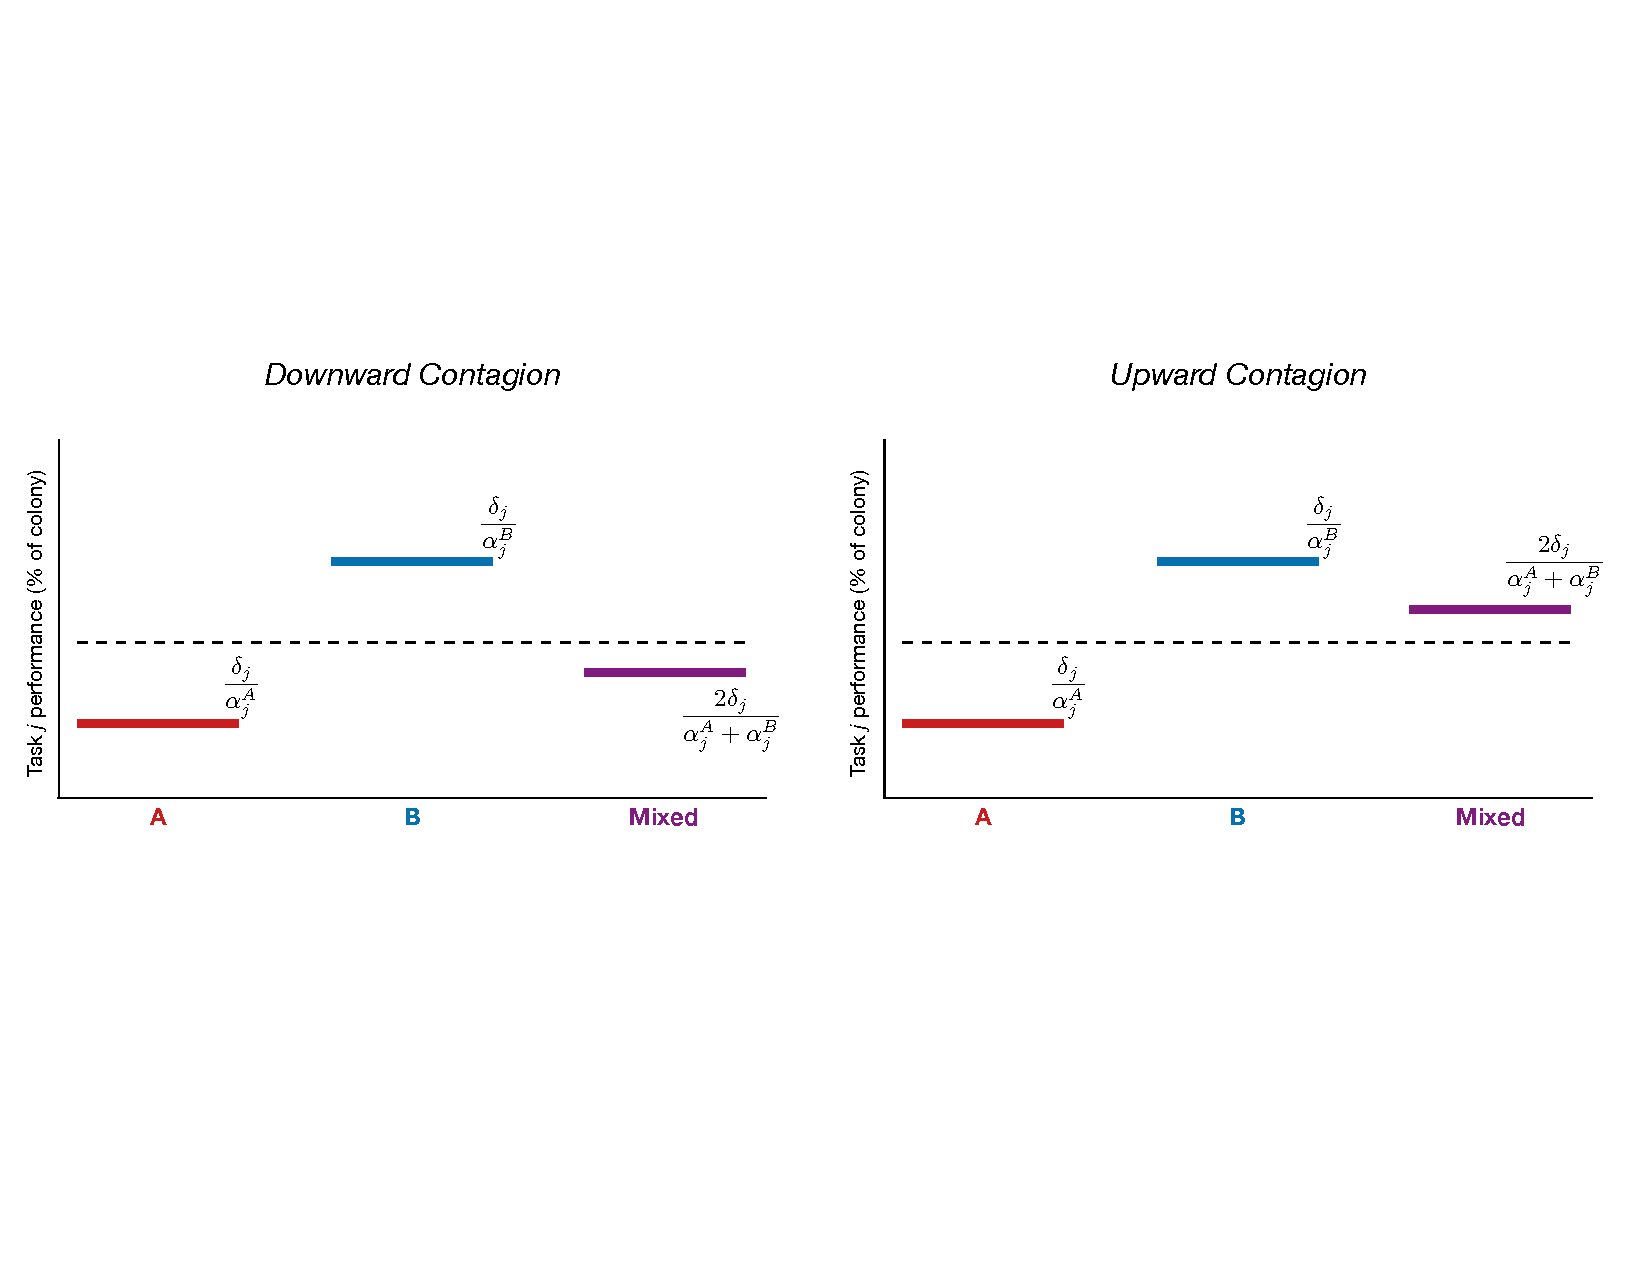
\includegraphics[width=0.9\linewidth]{doc/schematic_contagion.pdf}
    \caption{A schematic representing the two contagion patterns of our interest. The task $j$ performance (\%) values for the mixed colonies assume that the mean thresholds and the quit probabilities are identical for both lines and both tasks ($\mu_1^{\A} = \mu_2^{\A} = \mu_1^{\B} = \mu_2^{\B}$) and ($\tau^{\A} = \tau^{\B}$).}
    \label{fig:schematic}
\end{figure}
By manipulating the inequality \eqref{eq:down}, however, we see that \textbf{only the downward contagion is possible} under our assumptions:
\begin{align}
    \frac{1}{2} \bigg( \frac{\delta_j}{\alpha_j^{\A}} + \frac{\delta_j}{\alpha_j^{\B}} \bigg) - \frac{2\delta_j}{\alpha_j^{\A} + \alpha_j^{\B}} 
    & = \frac{\delta_j}{2} \bigg( \frac{1}{\alpha_j^{\A}} + \frac{1}{\alpha_j^{\B}} - \frac{4}{\alpha_j^{\A} + \alpha_j^{\B}} \bigg) \nonumber\\
    & = \frac{\delta_j}{2} \Bigg( 
    \frac{\alpha_j^{\B} (\alpha_j^{\A} + \alpha_j^{\B}) + \alpha_j^{\A} (\alpha_j^{\A} + \alpha_j^{\B}) - 4\alpha_j^{\A}\alpha_j^{\B}}{\alpha_j^{\A}\alpha_j^{\B}(\alpha_j^{\A} + \alpha_j^{\B})} \Bigg) \nonumber\\
    & = \frac{\delta_j}{2} \Bigg( 
    \frac{ (\alpha_j^{\A})^2 + (\alpha_j^{\B})^2 - 2\alpha_j^{\A}\alpha_j^{\B}}{\alpha_j^{\A}\alpha_j^{\B}(\alpha_j^{\A} + \alpha_j^{\B})} \Bigg) 
    = \frac{\delta_j}{2} \Bigg( 
    \frac{ (\alpha_j^{\A} - \alpha_j^{\B})^2 }{\alpha_j^{\A}\alpha_j^{\B}(\alpha_j^{\A} + \alpha_j^{\B})} \Bigg) > 0
\end{align}

Upward contagion is still possible if we relax some of our assumptions. In the simulations I've run so far, upward contagion appears
\begin{itemize}
    \item when the mean thresholds ($\mu$) are varied in addition to the task efficiencies ($\alpha$), or
    \item when at least one of the lines is not sufficiently efficient to maintain the stimuli at constant levels (i.e., reach steady state).
\end{itemize}

\section{Questions}
\begin{itemize}
    \item {\color{orange}Even when there is ample demand, the ants spend <90\% of the time performing the tasks. What mechanism explains the presence of this ``ceiling'' effect?}
    
    \item How reasonable is it to assume that the empirically observed behavior corresponds to the steady state of the model? {\color{orange}Need to make this assumption for steady-state analysis, but should also consider cases where this assumption does not hold and }
    
    \item From our earlier simulations, we know that both the mean threshold ($\mu$) or the quit probability ($\tau$) lead to ``behavioral amplification'' in the mixed case.
    Biologically speaking, which is more likely to vary by genetic line? Also, what happens when $\alpha$ AND either $\mu$ and $\tau$ are varied?
    
    \item What do these ``upward'' and ``downward'' contagions imply? As in, why might they be biologically interesting? {\color{orange}We will ask Yuko et al. when we send them the summary document.}
\end{itemize}

\begin{thebibliography}{99}

\bibitem{ulrich18} Y. Ulrich, J. Saragosti, C. K. Tokita, C. E. Tarnita, D. J. C. Kronauer, ``Fitness benefits and emergent division of labour at the onset of group living,'' \textit{Nature}, vol. 560, pp. 635-638, Aug. 2018.

\end{thebibliography}

\end{document}
%%%%%%%%%%%%%%%%%%%%%%%%%%%

